%\mag1440
%\mag600
%\documentclass[draft,a4paper,12pt,reqno,oneside]{amsart}
%\documentclass[final,a4paper,12pt,reqno,oneside]{amsart, extarticle}
\documentclass[final,a4paper,14pt,reqno,oneside]{extarticle}
%\documentclass[draft,a4paper,12pt,reqno]{amsart}
%\documentclass[12pt]{article}
%\usepackage[T1]{fontenc}
\usepackage{cmap}
\usepackage[utf8]{inputenc}
\usepackage[T2A]{fontenc}
\usepackage[T2B]{fontenc}
\usepackage[T2C]{fontenc}
\usepackage[russian]{babel}
%\input glyphtounicode
%\pdfgentounicode=1
\usepackage{amsmath}
\usepackage{amssymb}
\usepackage{verbatim}
\usepackage{wasysym}
\usepackage{longtable}
\usepackage[center]{titlesec}
%\usepackage{sectsty}
%\usepackage{epic}
%\usepackage{eepic}
\usepackage{epsfig}
%\usepackage{floatflt}
\usepackage{graphicx}
%\usepackage{chapterbib}
\usepackage[nottoc]{tocbibind}
\usepackage[russian]{cleveref}

%\newcommand{\crefmiddleconjunction}{, }
%\newcommand{\creflastconjunction}{ и~}
%\newcommand{\crefrangeconjunction}{--}
%\newcommand{\crefpairconjunction}{, }
\crefname{equation}{\!\!}{\!\!}
\crefname{figure}{\!\!}{\!\!}

\linespread{1.3}

\hoffset=-10mm
\textwidth=175 mm
\textheight=263 mm
\topmargin=-20 mm
\headheight=3 mm
\headsep=10 pt
\oddsidemargin=12 mm

%\setlength{\oddsidemargin}{5 mm} \setlength{\topmargin}{0 mm}
%\setlength{\headheight}{0 mm} \setlength{\headsep}{0 mm}
%\setlength{\textwidth}{160 mm} \setlength{\textheight}{240 mm}

%\tolerance=1000
%\pagestyle{empty}

\graphicspath{{./images/}}
 


%\DeclareMathAccent{\widetilde}{\mathord}{largesymbols}{"65}
%\DeclareMathAccent{\widetilde}{\mathrel}{largesymbols}{93}
%\DeclareMathAccent{\widetilde}{\mathrel}{largesymbols}{"12}
%\DeclareMathAccent{\widetilde}{\mathord}{letters}{"5F}
%\DeclareMathAccent{\widetilde}{\mathalpha}{AMSa}{"61}
\DeclareMathAccent{\widetilde}{\mathalpha}{largesymbols}{"45}
%\DeclareMathAccent{\widehat}{\mathord}{largesymbols}{"62}
\newcommand\ff{\varphi}
\renewcommand{\f}{\varphi}
\newcommand{\ft}{\tilde\varphi}
\newcommand\eps{\varepsilon}
%\newcommand{\e}{\varepsilon}
\newcommand{\Q}{\theta}
\newcommand{\Qt}{\tilde\theta}
\newcommand{\la}{\lambda}
\newcommand{\al}{\alpha}
\newcommand{\be}{\beta}
\newcommand{\ga}{\gamma}
\newcommand{\s}{\sigma}
\newcommand{\x}{\xi}
\newcommand{\z}{\zeta}
\renewcommand{\r}{\rho}
\newcommand{\rt}{\tilde\rho}
\newcommand{\n}{\eta}
\renewcommand{\t}{\tau}
\newcommand{\er}{\bar{e}_r}
\newcommand{\F}{\mathbf{\Phi}}
\newcommand{\hU}{\mathbf{\hat{U}}}
\renewcommand{\P}{\Psi}
\newcommand{\nab}{\nabla}
\newcommand{\Lap}{\Delta}
\newcommand\om{\omega}
\newcommand\Om{\Omega}
\newcommand\Gmm{\Gamma}
\renewcommand{\k}{\varkappa}
\newcommand\dss{\displaystyle}
\newcommand\fr{\frac}
\newcommand\df{\dfrac}
\newcommand\de{\partial}
\newcommand\Op{\operatorname}
\newcommand\idot{\,\cdot}
\renewcommand{\.}{\,\cdot\,} % index dot
\newcommand{\dotm}{\!\cdot\!} % dot for scalar multiple
\newlength{\ertp}
\newcommand{\No}{№}
\renewcommand{\rt}{\tilde r}
\newcommand{\todo}{\textbf}
%\renewcommand{\sectname}{Лекция }\sectname
%\renewcommand{\cite}[1]{}
%\renewcommand{\"}{\symbol{34}}
\def\q{\quad}
\def\qq{\qquad}
%\DeclareMathOperator\div{div}
%\DeclareMathOperator\det{det}
\DeclareMathOperator{\e}{e}
\DeclareMathOperator{\diver}{div}
\DeclareMathOperator{\grad}{grad}
\DeclareMathOperator{\rot}{rot}
\DeclareMathOperator{\dif}{d}
\newcommand\diff{\dif \!}
\DeclareMathOperator{\opL}{L}
\DeclareMathOperator{\T}{T}
\DeclareMathOperator{\const}{const}
\unitlength 1.0mm \linethickness{0.4pt}


\newcommand\equationF[3]{%
\begin{equation}{\label{#1}}
 \raisebox{#3pt}{\includegraphics[scale=#2]{FIGs/#1}}\ ,
\end{equation}
}%

\newcommand{\equationFnl}[3]{%
\begin{equation*}{\label{#1}}
 \raisebox{#3pt}{\includegraphics[scale=#2]{FIGs/#1}}\ ,
\end{equation*}
}%

\newcommand\equationFF[3]{$$\raisebox{#1pt}{#3}\eqno{(#2)}$$}%

\renewcommand\thesection{\arabic{section}.}
\renewcommand\thesubsection{\thesection\arabic{subsection}.}
\renewcommand\thesubsubsection{\thesubsection\arabic{subsubsection}.}
%\allsectionsfont{\centering}
\begin{document}

\makeatletter
%\renewcommand{\thesection}{}
\renewcommand{\@oddhead}{}
\renewcommand{\@oddfoot}{\hfil \thepage \hfil}
\renewcommand{\l@section}{\@dottedtocline{1}{0em}{2.3em}} %содержание
%\renewcommand{\l@section}[2]{\hbox to\textwidth{#1\dotfill #2}}
\makeatother

%\renewcommand{\bibname}{Список литературы к лекции}
%\renewcommand\refname{Какой-то список}

\newcommand{\ssection}[1]{%
  \section[#1]{\centering\normalfont\scshape #1}}
\newcommand{\ssubsection}[1]{%
  \subsection[#1]{\raggedright\normalfont\itshape #1}}

\setlength{\parindent}{1.0cm}

\setlength{\leftmargini}{1.0cm}
\def\theenumi{\arabic{enumi}}
\def\labelenumi{\theenumi)}

%\setlength{\par1}{\parindent}
%\setlength{\parskip}{1ex}
%\parskip=2pt\parindent 0pt
\setlength{\ertp}{\parindent}



\renewcommand{\bibname}{СПИСОК ИСПОЛЬЗОВАННЫХ ИСТОЧНИКОВ}
\renewcommand\refname{СПИСОК ИСПОЛЬЗОВАННЫХ ИСТОЧНИКОВ}

%\input{title.tex}

%\newpage
\setcounter{page}{2}
\thispagestyle {empty}
\renewcommand{\contentsname}{\centering СОДЕРЖАНИЕ}
\tableofcontents

\newpage
\section*{ВВЕДЕНИЕ}
\addcontentsline{toc}{section}{ВВЕДЕНИЕ}


Потребность в~изучении дифракции на~различных телах очень высока. Знания, полученные путем изучения дифракции с~помощью моделей, используются как в~гидроакустике и~эхолокации, так и~в~других областях. В~дефектоскопии основной задачей является обнаружение различных включений в~однородном теле. Это позволяет проводить исследование различных объектов методом неразрушающего контроля. Задача эхолокации~--- обнаружить и~определить местоположение объектов  по~времени задержки отражённой волны.

Для~современного мира изучение простых моделей уже не~дает требуемой точности прогнозирования поведения волн. Поэтому, необходимо изучать более сложные модели, детально описывающие рассматриваемые тела и~окружающую среду. Изучение тел с~произвольно расположенными полостями является более трудной задачей, по~сравнению с~классическими моделями. 

В~настоящей работе рассматривается задача дифракции плоских звуковых волн на~упругой сфере с произвольно расположенной полостью, заполненной жидкостью, и~радиально-неоднородным упругим покрытием. С~помощью таких покрытий можно изменять звукоотражающие свойства тел, что позволяет решать различные задачи по~формированию заданной дифракционной картины. Такой слой возможно сделать в~промышленных условиях, комбинируя несколько тонких однородных слоев с~различными механическими характеристиками. В~качестве рассматриваемого тела выбрана сфера, т.к. она является подходящей аппроксимацией для~большинства сложных тел. В~ходе работы получено аналитическое описание акустического поля, рассеяного телом, предложено решение полученной краевой задачи для~системы обыкновенных дифференциальных уравнений и~представлены результаты расчетов диаграмм направленности рассеянного поля и~частотных характеристик для~различных покрытий.


\newpage
\section{МАТЕМАТИЧЕСКОЕ МОДЕЛИРОВАНИЕ РАСПРОСТРАНЕНИЯ ЗВУКОВЫХ ВОЛН}

\newpage
\subsection{Распространение звука в идеальной жидкости}

Для математического процесса моделирования распространения звука в~идеальной среде воспользуемся полной системой уравнений гидромеханики идеальной жидкости, описывающей любые движения идеальной жидкости. Эта система включает уравнение движения идеальной жидкости (уравнение Эйлера), уравнение неразрывности и~уравнение физического состояния.

Математическое описание движения жидкости осуществляется с~помощью функций, определяющих распределение скорости~$\bar{v}$, давления~$P$ и~плотности~$p$. Уравнение Эйлера имеет вид
\begin{equation}\label{eq1}
\fr{\de \bar{v}}{\de t} + (\bar{v} \cdot \nab)\bar{v} = \bar F - \fr{1}{p}\grad P,
\end{equation}
где $\bar F$ --- массовая сила, отнесённая к~единице массы.

Уравнение неразрывности записывается в~виде
\begin{equation}\label{eq2}
\fr{\de \bar{p}}{\de t} + \diver (p \bar{v}) = 0.
\end{equation}

Будем считать, что движение сжимаемой жидкости происходит адиабатически. В~этом случае уравнение физического состояния принимает вид
\begin{equation}\label{eq3}
P=P_0\bigg(\fr{p}{p_0}\bigg)^\gamma, \qq \gamma=\fr{C_P}{C_V}
\end{equation}
где $P_0$ и $p_0$ --- давление и~плотность невозмущенной жидкости; \\
 $C_P$ и $C_V$ --- теплоемкость при~постоянном давлении и~постоянном объеме.

Процесс распространения звука представляет собой малые колебания жидкости, так что в~уравнении \eqref{eq1} можно пренебречь конвективными членами. Полагая, что~внешние силы отсутствуют, получим:
\begin{equation}\label{eq4}
\fr{\de \bar{v}}{\de t} = - \fr{1}{p}\grad P.
\end{equation}
Введем в~рассмотрение величину~$s$, называемую сжатием и~равную относительному изменению плотности
\begin{equation}\label{eq5}
s=\fr{p - p_0}{p_0}; \qq p = p_0 (1+s).
\end{equation}

Тогда уравнение \eqref{eq3} перепишем в~виде
\begin{equation}\label{eq6}
P=P_0(1+s)^\gamma.
\end{equation}
При малых колебаниях жидкости сжатие~$s$ настолько мало, что~высшими степенями~$s$ можно пренебречь. В~результате из~выражения~\eqref{eq6} получим
\begin{equation}\label{eq7}
P=P_0(1+\gamma \cdot s).
\end{equation}

Подставим выражение~\eqref{eq5} в~уравнение неразрывности. Так как 
$$
\diver(p \bar{v})= p\diver(\bar{v})+\bar{v} \grad p = p_0 \diver(\bar{v}) + p_0 s \diver(\bar{v}) + \bar{v} \grad p,
$$
причем последними двумя слагаемыми можно пренебречь, то~вместо уравнения~\eqref{eq2} будем иметь
\begin{equation}\label{eq8}
\fr{\de s}{\de t} + \diver (\bar{v}) = 0.
\end{equation}
Уравнение \eqref{eq4} в~том~же приближении сводится к~уравнению
\begin{equation}\label{eq9}
\fr{\de \bar{v}}{\de t} = -c^2\cdot\grad s,
\end{equation}
где $c=\sqrt{\gamma \fr{P_0}{p_0}}$ --- скорость звука.

Предположим теперь, что~в~начальный момент существует потенциал скоростей~$\tilde\P_0$, т.е.
\begin{equation}\label{eq 10}
\bar{v}\big|_{t=0}=\grad\tilde\P_0.
\end{equation}

Из~уравнения~\eqref{eq9} имеем
$$
\bar{v}=\bar{v}\big|_{t=0}-c^2\grad \bigg(\int\limits_{0}^{t} s\diff t\bigg).
$$
С~учетом~\eqref{eq 10} получаем
\begin{equation}\label{eq 11}
\bar{v}=\grad\bigg[\tilde\P_0-c^2\int\limits_{0}^{t} s\diff t\bigg]=\grad\tilde\P.
\end{equation}
Это означает, что~существует потенциал скоростей~$\tilde\P$ в~любой момент времени~$t:$
$$
\tilde\P=\tilde\P_0-c^2\int\limits_{0}^{t} s\diff t.
$$

Дифференцируя последнее выражение два~раза по~$t,$ получим
\begin{equation}\label{eq 12}
\fr{\de^2\tilde\P}{\de t^2}=-c^2\fr{\de s}{\de t}.
\end{equation}

С~другой стороны, подставляя выражение~\eqref{eq 11} в~уравнение~\eqref{eq8}, будем иметь
\begin{equation}\label{eq 13}
\fr{\de s}{\de t}=-\diver\grad\tilde\P=-\Lap\tilde\P.
\end{equation}
Из~уравнений~\eqref{eq 12} и~\eqref{eq 13} приходим к~волновому уравнению
\begin{equation}\label{eq 14}
\fr{\de^2\tilde\P}{\de t^2}=c^2\Lap\tilde\P,
\end{equation}
которое описывает процесс распространения звука в~идеальной жидкости.

Отметим, что~знания потенциала~$\tilde\P$ достаточно для~определения всего процесса движения жидкости в~случае малых возмущений, так~как
$$
\bar{v}=\grad\tilde\P;\qq s=-\fr{1}{c^2}\fr{\de\tilde\P}{\de t}.
$$

Найдем акустическое давление~$P'=P-P_0$. Из~уравнения~\eqref{eq4}, используя приближение, сделанное для~\eqref{eq9}:
$$
\fr{\de \grad \tilde\P}{\de t} = - \fr{1}{p_0}\grad P'.
$$

Занесем дифференциал под~градиент и~перенесем в~левую часть:
$$
\grad \left(\fr{\de \tilde\P}{\de t} + \fr{P'}{p_0}\right) = 0.
$$
Выражение в~скобках не~зависит от~координат. Учитывая, что~потенциал~$\tilde\P$ определяется с~точностью до~функции времени, приравняем выражение в~скобках нулю:
$$
\fr{\de \tilde\P}{\de t} + \fr{P'}{p_0} = 0.
$$

В~случае установившегося режима колебаний
\begin{equation}\label{eq 15}
\tilde\P=\P \e^{-i\om t}
\end{equation}
уравнение~\eqref{eq 14} переходит в~уравнение Гельмгольца
\begin{equation}\label{eq 16}
\Lap{\P}+k^2\P=0,
\end{equation}
где $\om$ --- круговая частота; $k=\fr{\om}{c}$ --- волновое число.
При~этом акустическое давление 
$$
P'=-p_0 \fr{\de \tilde\P}{\de t}=-p_0 \cdot (-i \om) \P \e^{-i\omega t}=ip_0\om\tilde{\P}.
$$


\newpage
\subsection{Распространение звуковых волн в упругих телах}

\todo{Ландау - Теория упругости, Амензаде}
\todo{моделирование волновых полей}

\newpage
\section{ДИФРАКЦИЯ ЗВУКОВЫХ ВОЛН НА УПРУГОЙ СФЕРЕ, ИМЕЮЩЕЙ ПРОИЗВОЛЬНО РАСПОЛОЖЕННУЮ ПОЛОСТЬ И НЕОДНОРОДНОЕ ПОКРЫТИЕ}

\newpage
\subsection{Обзор литературы по проблеме исследования}
\todo{Известия ТулГУ №3 Ларин; статьи Толоконникова}

\newpage
\subsection{Постановка задачи}
\begin{figure}[h]
\begin{center}
\begin{minipage}[h]{0.47\linewidth}
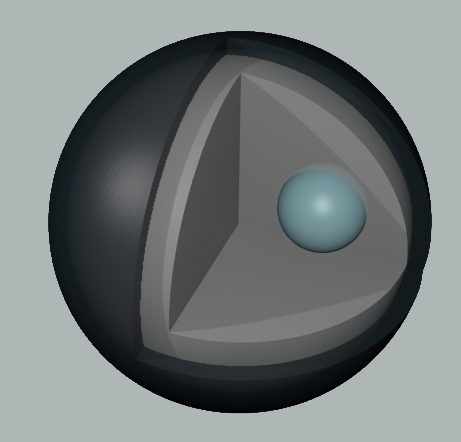
\includegraphics[width=1\linewidth]{sphere_edited.png}
\caption{<<Сфера со сферическим слоем и произвольно расположенной сферической полостью>>}\label{pic_1}
\end{minipage}
%\hfill
%\begin{minipage}[h]{0.47\linewidth}
%\includegraphics[width=1\linewidth]{2a}
%\caption{<<при $ka=3.2$>>}
%\end{minipage}
\end{center}
\end{figure}

Рассмотрим изотропный однородный упругий шар радиуса~$R\s$, плотность материала которого~$p\s$, упругие постоянные~$\la\s$ и~$\mu\s$, содержащий произвольно расположенную сферическую полость с~радиусом~$R\c$. Шар имеет покрытие в~виде неоднородного изотропного упругого слоя, внешний радиус которого равен~$R\l$ (рис. \cref{pic_1}).
 
Свяжем с полостью тела и с~самим телом прямоугольные системы координат $x\c, y\c, z\c$ и $x\s, y\s, z\s$ соответственно так, чтобы соответствующие оси обеих систем координат были параллельны. С~декартовыми системами координат $x\c, y\c, z\c$ и $x\s, y\s, z\s$ свяжем сферические координаты $r\c, \Q\c, \f\c$ и $r\s, \Q\s, \f\s$.

Пусть модули упругости~$\la\l$ и~$\mu\l$ материала слоя описываются дифференцируемыми функциями радиальной координаты~$r\s$ сферической системы координат~$(r\s, \Q\s, \f\s)$, а плотность $p\l$~--- непрерывной функцией координаты~$r\s$.  Окружающая тело и находящаяся в его полости жидкости~--- идеальные и однородные, имеющие плотности~$p\en, p\c$ и скорости звука~$c\en, c\c$ соответственно. 

Определим отраженные от~тела и возбужденные в~его~полости волны, а также найдем поля смещений в~упругом материале шара и неоднородном слое.


\newpage
\subsection{Аналитическое решение задачи}

Пусть из~внешнего пространства на~шар падает плоская звуковая волна. Потенциал скоростей гармонической падающей волны запишем в~виде:
\begin{equation}\label{potential speed}
\P\o(\bar{x}\s, t) = A\o \exp\left[i\left(\bar{k}\en\dotm\bar{x}\s-\om t\right)\right],
\end{equation}
где $A\o$~--- амплитуда волны, \\
$\bar{k}_e$~--- волновой вектор в~окружающей жидкости,  \\
$\lvert\bar{k}\en\rvert = k\en = \om / c\en$~--- волновое число, \\
$\bar{x}\s$~--- радиус-вектор, \\
$\om$~--- круговая частота.

 Без~ограничения общности будем полагать, что волна распространяется в~направлении~$\Q\s = \Q\c = 0$. Тогда в~сферической системе координат \eqref{potential speed} запишется в~виде:
\begin{equation}\label{potential speed theta = 0}
\P\o(r\s, \Q\s, t) = A\o \exp\left[i\left(k\en r\s\cos\Q\s - \om t\right)\right],
\end{equation}
В~дальнейшем временной множитель~$\exp(-i\om t)$ будем опускать.

Разложим \eqref{potential speed theta = 0} в ряд по ортогональным функциям:
\begin{equation}
\P\o(r\s, \Q\s, f\s) = \sum\limits_{n=0}^\infty\sum\limits_{m=-n}^n \gamma_{mn}j_n(k\en r\s)P_n^{\lvert m\rvert}(\cos\Q\s)\e^{im\f\s},
\end{equation}
где $j_n(x)$~--- сферическая функция Бесселя порядка $n;$\\
$P_n^m(x)$~--- присоединенный многочлен Лежандра степени $n$ порядка $m;$\\
$\gamma_{mn} = 
\begin{cases}
A\o i^n(2n+1),& \text{при } m=0;\\
0,& \text{при } m \ne 0.
\end{cases}
$

Задача определения акустических полей вне~упругого тела и внутри его~полости в~установившемся режиме колебаний заключается в~нахождении решений уравнения Гельмгольца:
\begin{align}
\Lap\P\en &+ k\en^2\P\en = 0;\label{Helmholtz_ambient}\\
\Lap\P\c &+ k\c^2\P\c = 0,\label{Helmholtz_hollow}
\end{align}
где $\P\en$~--- потенциал скоростей полного акустического поля во~внешней среде;\\
$\P\c$~--- потенциал скоростей акустического поля в~полости тела;\\
$k\c = \df{\om}{c\c}$~--- волновое число находящейся в~полости жидкости.\\ При~этом скорости частиц жидкости и акустическое давление вне~тела и внутри полости определяются по~следующим формулам соответственно:
\begin{align}
\v\en &= \grad\P\en; &\q P\en &= ip\en\om\P\en;\label{eq_ven}\\
\v\c &= \grad\P\c; &\q P\c &= ip\c\om\P\c.\label{eq_vc}
\end{align}


В~силу линейной постановки задачи для $\P\en$ и $\P\o$ справедливо
\begin{equation} \label{potention_speed_ambient}
\P\en = \P\o + \P\sc,
\end{equation}
где $\P\sc$~--- потенциал скоростей рассеянной звуковой волны.\\
Тогда из~\eqref{Helmholtz_ambient} получаем уравнение для нахождения~$\P\sc$:
\begin{equation} \label{Helmholtz_ambient_diffraction}
\Lap\P\sc + k\en^2\P\sc = 0.
\end{equation}

Из-за~произвольного расположения полости в теле потенциалы $\P\c$ и $\P\sc$ не~будут проявлять свойства симметрии.
Уравнения~\cref{Helmholtz_hollow,Helmholtz_ambient_diffraction} запишем в~сферических системах координат~$(r\c, \Q\c, \f\c)$ и $(r\s, \Q\s, \f\s)$ соответственно:
\begin{align}
\fr1{r\c^2}\fr\de{\de r\c}\left(r\c^2 \fr{\de\P\c}{\de r\c}\right) + \fr1{r\c^2\sin^2\Q\c}\fr{\de\P\c}{\de\f\c^2} &+ \fr1{r\c^2\sin\Q\c}\fr\de{\de\Q\c} \left(\sin\Q\c \fr{\de\P\c}{\de\Q\c}\right) + k\c^2\P\c = 0;\\
\fr1{r\s^2}\fr\de{\de r\s}\left(r\s^2 \fr{\de\P\sc}{\de r\s}\right) + \fr1{r\s^2\sin^2\Q\s}\fr{\de\P\sc}{\de\f\s^2} &+ \fr1{r\s^2\sin\Q\s}\fr\de{\de\Q\s} \left(\sin\Q\s \fr{\de\P\sc}{\de\Q\s}\right) + k\en^2\P\sc = 0.
\end{align}

Звуковая волна в~полости тела~$\P\c$ должна удовлетворять условию ограниченности, а отраженная волна~$\P\sc$~--- условиям излучения на~бесконечности. Поэтому потенциалы $\P\sc$ и $\P\c$ будем искать в~виде рядов по сферическим функциям:
\begin{align}\P\sc(r\s, \Q\s, \f\s) &= \sum\limits_{n = 0}^\infty \sum\limits_{m = 0}^n {A\sc}_{nm} h_n(k\en r\s) P_n^{\lvert m\rvert}(\cos\Q\s)\cos\bigl(m\f\s\bigr);\label{eq_psc}\\
\P\c(r\c, \Q\c, \f\c) &= \sum\limits_{n = 0}^\infty \sum\limits_{m = 0}^n {B\c}_{nm} j_n(k\c r\c) P_n^{\lvert m\rvert}(\cos\Q\c)\cos\bigl(m\f\c\bigr),\label{eq_pc}
\end{align}
где $h_n(x)$~--- сферическая функции Ханкеля первого рода.

Распространение малых возмущений в~упругом теле для~установившегося режима движения частиц тела описывается скалярным и векторным уравнением Гельмгольца:
\begin{align}
\Lap\P\s &+ {k\s}_l^2\P\s = 0;\label{Helmholtz_scalar}\\
\Lap\F\s &+ {k\s}_\t^2\F\s = 0,\label{Helmholtz_vector}
\end{align}
где ${k\s}_l$~--- волновое число продольных волн со~скоростью распространения \break 
${c\s}_l = \sqrt{\df{(\la\s + 2\mu\s)}{p\s}}$;\\
${k\s}_\t$~--- волновое число поперечных волн со~скоростью распространения \\
${c\s}_\t = \sqrt{\df{\mu\s}{p\s}}$;\\
$\P\s$ и $\F\s$~--- скалярной и векторный потенциалы смещения соответственно.

Вектор смещения $\u\s$ частиц упругого тела определяется по~формуле
$$
\u\s = \grad \P\s + \rot \F\s.
$$

Потенциал смещения $\P\s$ будем искать в~виде ряда по~двум локальным сферическим функциям:
\begin{equation}\label{eq_ps}
\begin{split}
\P\s = \sum\limits_{n=0}^\infty \sum\limits_{m=-n}^n 
  &{A\s}_{nm} h_n({k\s}_lr\c)P_n^{\lvert m\rvert}(\cos\Q\c)\e^{im\f\c} +\\
+ &{B\s}_{nm} j_n({k\s}_lr\s)P_n^{\lvert m\rvert}(\cos\Q\s)\e^{im\f\s}
\end{split}
\end{equation}

Векторный потенциал $\F\s$ может быть представлен в~виде суммы:
$$
\F\s = rV\er + \rot\bigl(rW\er\bigr),
$$
где $\er$~--- орт координатной оси~$r\s$ сферической системы координат~$r\s, \Q\s, \f\s,$\\
функции $V$ и $W$ удовлетворяют скалярным уравнениям Гельмгольца
\begin{align}
\Lap V &+ {k\s}_\t^2 V = 0,\\
\Lap W &+ {k\s}_\t^2 W = 0.
\end{align}

Компоненты вектора $\u\s$ выражаются через функции $\P\s, V$ и $W$ следующим образом:
\begin{equation}\label{eq_us}
\begin{split}
{u\s}_r &= \fr{\de \P\s}{\de r\s} - \fr{1}{r\s}L(W),\\
{u\s}_\Q &= \fr{1}{r\s}\fr{\de \P\s}{\de \Q\s} + \fr{1}{r\s}\fr{\de}{\de r\s}\left(r\s\fr{\de W}{\de \Q\s}\right) + \fr{1}{\sin\Q\s}\fr{\de V}{\de\f\s},\\
{u\s}_\f &= \fr{1}{r\s \sin\Q\s}\fr{\de \P\s}{\de \f\s} + \fr{1}{r\s\sin\Q\s}\fr{\de}{\de r\s}\left(r\s\fr{\de W}{\de \f\s}\right) - \fr{\de V}{\de \Q\s},
\end{split}
\end{equation}
где $L = \df{\de^2}{\de\Q\s^2} + \ctg\Q\s\df{\de}{\de\Q\s} + \df{1}{\sin^2\Q\s}\df{\de^2}{\de\f\s^2}.$

Функции $V$ и $W$ будем искать в~виде:
\begin{align}
V = \sum\limits_{n=0}^\infty \sum\limits_{m=-n}^n &{C\s}_{nm} h_n({k\s}_lr\c)P_n^{\lvert m\rvert}(\cos\Q\c)\e^{im\f\c} + \notag\\
+ &{D\s}_{nm} j_n({k\s}_lr\s)P_n^{\lvert m\rvert}(\cos\Q\s)\e^{im\f\s},\label{eq_v}\\
W = \sum\limits_{n=0}^\infty \sum\limits_{m=-n}^n &{E\s}_{nm} h_n({k\s}_lr\c)P_n^{\lvert m\rvert}(\cos\Q\c)\e^{im\f\c} + \notag\\
+ &{F\s}_{nm} j_n({k\s}_lr\s)P_n^{\lvert m\rvert}(\cos\Q\s)\e^{im\f\s}.\label{eq_w}
\end{align}

Распространение упругих волн в неоднородном слое описывается общими уравнениями движения упругой среды, которые для установившегося режима движения в сферической системе координат имеют следующий вид~\cite{Nowacki}:
\begin{equation}\label{eq_moving}
\begin{split}
\fr{\de{\si\l}_{rr}}{\de r\s} &+ \fr1{r\s} \fr{\de{\si\l}_{r\Q}}{\de\Q\s} + \fr{1}{r\s\sin\Q\s}\fr{\de\si_{r\f}}{\de\f} +\\
&+ \fr1{r\s}\biggl(2{\si\l}_{rr}-{\si\l}_{\Q\Q}-{\si\l}_{\f\f}+{\si\l}_{r\Q}\ctg\Q\s\biggr)=-p\l\om^2{u\l}_r;\\
\fr{\de{\si\l}_{r\Q}}{\de r\s} &+ \fr1{r\s} \fr{\de{\si\l}_{\Q\Q}}{\de\Q\s} + \fr{1}{r\s\sin\Q\s}\fr{\de{\si\l}_{\Q\f}}{\de\f\s} +\\
&+ \fr1{r\s}\biggl(\left({\si\l}_{\Q\Q}-{\si\l}_{\f\f}\right)\ctg\Q\s+3{\si\l}_{r\Q}\biggr)\!=\!-p\l\om^2{u\l}_\Q;\\
\fr{\de{\si\l}_{r\f}}{\de r\s} &+ \fr1{r\s} \fr{\de{\si\l}_{\Q\f}}{\de\Q\s} + \fr{1}{r\s\sin\Q\s}\fr{\de{\si\l}_{\f\f}}{\de\f\s} +\\
&+ \fr1{r\s}\biggl(3{\si\l}_{r\f}+2{\si\l}_{\Q\f}\ctg\Q\s\biggr)=-p\l\om^2{u\l}_\f,
\end{split}
\end{equation}
где ${u\l}_r, {u\l}_\Q, {u\l}_\f$ --- компоненты вектора смещения $\u\l$;\\
${\si\l}_{ij}$ --- компоненты тензора напряжений неоднородной среды в сферической системе координат.

Используя связь компонентов тензора напряжений с компонентами тензора деформаций (обобщенный закон Гука), а также выражения компонентов тензора деформаций через компоненты вектора смещения~\cite{Nowacki}, получаем в сферической системе координат следующие соотношения:
\begin{equation}\label{tensor comp}
    \begin{gathered}
    \begin{aligned}
        {\si\l}_{rr} &= \biggl(\la\l+2\mu\l\biggr)\fr{\de {u\l}_r}{\de r\s} +\\
        &+ \fr{\la\l} {r\s} \biggl(2{u\l}_r+\fr{\de {u\l}_\Q}{\de\Q\s}+\ctg\Q\s\;{u\l}_\Q + \fr{1}{\sin\Q\s}\fr{\de {u\l}_\f}{\de\f\s}\biggr);\\        
        {\si\l}_{\Q\Q} &= \la\l\fr{\de {u\l}_r}{\de r\s} + \fr{2(\la\l+\mu\l)}{r\s} {u\l}_r + \fr{\la\l+2\mu\l}{r\s} \fr{\de {u\l}_\Q}{\de\Q\s} +\\
         &+ \fr{\la\l}{r\s} \biggl(\ctg\Q\s \;{u\l}_\Q + \fr{1}{\sin\Q\s}\fr{\de {u\l}_\f}{\de\f\s}\biggr);\\
        {\si\l}_{\f\f} &= \la\l\fr{\de {u\l}_r}{\de r\s} + \fr{2(\la\l+\mu\l)}{r\s} {u\l}_r + \fr{\la\l}{r\s} \fr{\de {u\l}_\Q}{\de\Q\s} +\\
        &+ \fr{\la\l+2\mu\l}{r\s}\biggl(\ctg\Q\s \;{u\l}_\Q + \fr{1}{\sin\Q\s}\fr{\de {u\l}_\f}{\de\f\s}\biggr);\\
    \end{aligned}\\
    \begin{aligned}
        {\si\l}_{r\Q}=\mu\l&\left(\fr1{r\s} \fr{\de {u\l}_r}{\de\Q\s} - \fr{{u\l}_\Q}{r\s} + \fr{\de {u\l}_\Q}{\de r}\right);\\
        {\si\l}_{r\f}=\mu\l&\left(\fr1{r\s\sin\Q\s} \fr{\de {u\l}_r}{\de\f} - \fr{{u\l}_\f}{r\s} + \fr{\de {u\l}_\f}{\de r\s}\right);\\
        {\si\l}_{\Q\f}=\fr{\mu\l} {r\s}&\left(\fr1{\sin\Q\s} \fr{\de {u\l}_\Q}{\de\f\s} + \fr{\de {u\l}_\f}{\de\Q\s} - \ctg\Q\s \;{u\l}_\f \right).\\
    \end{aligned}
    \end{gathered}
\end{equation}

Соотношения \eqref{tensor comp} справедливы как для однородной упругой среды, так и для неоднородного слоя. В первом случае в выражениях \eqref{tensor comp} компоненты вектора смещения $\u\l$ и тензора напряжений $\si\l,$ а также величины $\la\l$ и $\mu\l$ следует заменить на $\u\s, \si\s, \la\s$ и $\mu\s$ соответственно.

Используя эти соотношения, запишем уравнения~\eqref{eq_moving} через компоненты вектора смещения $\u\l$:
\begin{equation*}
\begin{split}
\biggl(\la\l+2\mu\l\biggr)\fr{\de^2 {u\l}_r}{\de r\s^2} + \fr{\mu\l}{r\s^2}\fr{\de^2 {u\l}_r}{\de\Q\s^2} +\fr{\mu\l}{r\s\sin\Q\s}\fr{\de^2 {u\l}_r}{\de\f\s^2} + \fr{\mu\l\ctg\Q\s}{r\s^2}\fr{\de {u\l}_r}{\de \Q\s} + \\
+ \left(\la\l'+2\mu\l'+\fr{2\la\l+4\mu\l}{r\s}\right)\fr{\de{u\l}_r}{\de r\s} + \left(\fr{2\la\l'}{r\s} - \fr{2\la\l+4\mu\l}{r\s^2}\right){u\l}_r + \\
+ \fr{\la\l+\mu\l}{r\s}\fr{\de^2 {u\l}_\Q}{\de r\s\de\Q\s} + \fr{(\la\l+\mu\l)\ctg\Q\s}{r\s}\fr{\de {u\l}_\Q}{\de r\s} + \\ 
+ \left(\fr{\la\l'}{r\s} - \fr{\la\l+3\mu\l}{r\s^2}\right)\fr{\de {u\l}_\Q}{\de \Q\s} +\left(\fr{\la\l'\ctg\Q\s}{r\s} - \fr{(\la\l+3\mu\l)\ctg\Q\s}{r\s^2}\right){u\l}_\Q + \\
+\fr{\la\l+\mu\l}{r\s\sin\Q\s}\fr{\de^2 {u\l}_\f}{\de r\s\de\f\s}
+ \left(\fr{\la\l'}{r\s\sin\Q\s} - \fr{\la\s+3\mu\s}{r\s^2\sin\Q\s}\right)\fr{\de {u\l}_\f}{\de \f\s} = -p\l\om^2{u\l}_r;
\end{split}
\end{equation*}

\begin{equation*}
\begin{split}
\fr{\la\l+\mu\l}{r\s}\fr{\de^2 {u\l}_r}{\de r\s \de \Q\s} + \left(\fr{\mu\l'}{r\s}+\fr{2\la\l+4\mu\l}{r\s^2}\right)\fr{\de {u\l}_r}{\de \Q\s} + \\
+ \mu\l \fr{\de^2 {u\l}_\Q}{\de r\s^2} + \fr{\la\l+2\mu\l}{r\s^2}\fr{\de^2 {u\l}_\Q}{\de \Q\s^2} + \fr{\mu\l}{r\s^2\sin^2\Q\s} \fr{\de^2 {u\l}_\Q}{\de \f^2} + \\
+ \left(\mu\l'+ \fr{2\mu\l}{r\s}\right)\fr{\de {u\l}_\Q}{\de r\s} + \fr{(\la\l+2\mu\l)\ctg\Q\s}{r\s^2}\fr{\de{u\l}_\Q}{\de \Q\s}-\left(\fr{\mu\l'}{r\s} + \fr{\la\l+2\mu\l}{r\s^2\sin^2\Q\s}\right){u\l}_\Q + \\
+ \fr{\la\l+\mu\l}{r\s^2\sin\Q\s}\fr{\de^2{u\l}_\f}{\de \Q\s \de \f\s} - \fr{(\la\l+3\mu\l)\ctg\Q\s}{r\s^2\sin\Q\s}\fr{\de {u\l}_\f}{\de \f\s}  = -p\l\om^2{u\l}_\Q;
\end{split}
\end{equation*}

\begin{equation*}
\begin{split}
\fr{\la\l+\mu\l}{r\s\sin\Q\s} \fr{\de^2{u\l}_r}{\de r\s \de \f\s} + \left(\fr{\mu\l'}{r\s\sin\Q\s} + \fr{2\la\l+4\mu\l}{r\s^2\sin\Q\s} \right)\fr{\de {u\l}_r}{\de \f\s} +\\
+ \fr{\la\l+\mu\l}{r\s^2\sin\Q\s}\fr{\de^2 {u\l}_\Q}{\de \Q\s \de \f\s} + \fr{(\la\l+3\mu\l)\ctg\Q\s}{r\s^2\sin\Q\s}\fr{\de {u\l}_\Q}{\de \f\s} +\\
+ \mu\l \fr{\de^2 {u\l}_\f}{\de r\s^2} + \fr{\mu\l}{r\s^2}\fr{\de^2 {u\l}_\f}{\de \Q\s^2} + \fr{\la\l+2\mu\l}{r\s^2\sin^2\Q\s} \fr{\de^2 {u\l}_\f}{\de \f\s^2} + \\
+ \left(\mu\l'+\fr{2\mu\l}{r\s}\right)\fr{\de {u\l}_\f}{\de r\s} + \fr{\mu\l\ctg\Q\s}{r\s^2}\fr{\de {u\l}_\f}{\de \Q\s} - \left(\fr{\mu\l'}{r\s} + \fr{\mu\l}{r\s^2\sin^2\Q\s}\right){u\l}_\f = - p\l\om^2{u\l}_\f.
\end{split}
\end{equation*}
Введем новые функции ${u\l}_2$ и ${u\l}_3$, связанные с ${u\l}_\Q$ и ${u\l}_\f$ следующими соотношениями:
\begin{equation}\label{eq_v2v3}
{u\l}_\Q = \df{\de {u\l}_2}{\de\Q\s} + \fr1{\sin\Q\s}\fr{\de {u\l}_3}{\de\f\s}; \qq {u\l}_\f = \df1{\sin\Q\s}\df{\de {u\l}_2}{\de\f\s} - \df{\de {u\l}_3}{\de\Q\s},
\end{equation}
запишем уравнения движения через функции ${u\l}_r, {u\l}_2$ и ${u\l}_3$ и перенесем всё в левую часть:

\begin{equation}\label{eq_1.1}
\begin{split}
\biggl(\la\l+2\mu\l\biggr)\fr{\de^2 {u\l}_r}{\de r\s^2} + \left(\la\l'+2\mu\l'+\fr{2\la\l+4\mu\l}{r\s}\right)\fr{\de {u\l}_r}{\de r\s} + \fr{\mu\l}{r\s^2}L({u\l}_r) +\\
+ \left(\fr{2\la\l'}{r\s} - \fr{2\la\l+4\mu\l}{r\s^2} + p\l\om^2\right){u\l}_r +\\
+ \left[\fr{\la\l+\mu\l}{r\s}\fr{\de}{\de r\s} + \fr{\la\l'}{r\s} - \fr{\la\l+3\mu\l}{r\s}\right]L({u\l}_3) = 0;
\end{split}
\end{equation}
\begin{equation}\label{eq_2.1}
\begin{split}
\left[\fr{\la\l+\mu\l}{r\s}\fr{\de}{\de r\s}+\fr{\mu\l'}{r\s}+\fr{2\la\l+4\mu\l}{r\s^2}\right]\fr{\de{u\l}_r}{\de \Q\s} + \fr{\la\l+2\mu\l}{r\s^2}\fr{\de}{\de \Q\s}L({u\l}_2) + \\
+ \left[\mu\l\fr{\de^2}{\de r\s^2} + \left(\mu\l'+\fr{2\mu\l}{r\s}\right)\fr{\de}{\de r\s} - \fr{\mu\l'}{r\s} + p\l\om^2\right]\left[\fr{\de {u\l}_2}{\de\Q\s} + \fr{1}{\sin\Q\s}\fr{\de{u\l}_3}{\de\f\s}\right]+\\
+ \fr{\mu\l}{r\s^2\sin\Q\s}\fr{\de}{\de\f\s}L({u\l}_3) = 0;
\end{split}
\end{equation}
\begin{equation}\label{eq_3.1}
\begin{split}
\fr{1}{r\s\sin\Q\s}\left[\biggl(\la\l+\mu\l\biggr)\fr{\de}{\de r\s} + \mu\l' + \fr{2\la\l+4\mu\l}{r\s}\right]\fr{\de {u\l}_r}{\de\f\s} +\\
+ \left[\mu\l\fr{\de^2}{\de r\s^2} + \left(\mu\l'+\fr{2\mu\l}{r\s}\right)\fr{\de}{\de r\s} - \fr{\mu\l'}{r\s} + p\l\om^2\right]\left[\fr{1}{\sin\Q\s}\fr{\de {u\l}_2}{\de\f\s} - \fr{\de {u\l}_3}{\de\Q\s}\right] +\\
+ \fr{\la\l+2\mu\l}{r\s^2\sin\Q\s}\fr{\de}{\de \f\s}L({u\l}_2) -\fr{\mu\l}{r\s^2}\fr{\de}{\de\Q\s}L({u\l}_3) = 0,
\end{split}
\end{equation}
где $\la\l' = \df{\diff\la\l}{\diff r\s},\q\mu\l' = \df{\diff\mu\l}{\diff r\s}.$

Сделаем преобразования уравнений. Уравнение \cref{eq_2.1} домножим на $\sin(\Q\s)$ и продифференцируем по $\Q\s$, а уравнение \cref{eq_3.1} продифференцируем по $\f\s.$ Сложим полученные уравнения и разделим на $\sin(\Q\s)$. Получим следующее уравнение:
\begin{equation}\label{eq_2.2}
\begin{split}
\left[\fr{\la\l+\mu\l}{r\s}\fr{\de}{\de r\s} + \fr{\mu\l'}{r\s} + \fr{2\la\l+4\mu\l}{r\s^2}\right]&L({u\l}_r)+\\
\left[\mu\l\fr{\de^2}{\de r\s^2} + \left(\mu\l'+\fr{2\mu\l}{r\s}\right)\fr{\de}{\de r\s} - \fr{\mu\l'}{r\s} + p\l\om^2\right]&L({u\l}_2) + \\
 + \fr{\la\l+2\mu\l}{r\s^2}&L^2({u\l}_2) = 0,
\end{split}
\end{equation}
не содержащее функцию ${u\l}_3.$ Затем продифференцируем уравнение \cref{eq_2.1} по $\f\s$ и вычтем уравнение \cref{eq_3.1}, предварительно умноженное на $\sin(\Q\s)$ и продифференцированное по $\Q\s,$ а затем всё разделим на $\sin(\Q\s).$ Получим следующее уравнение:
\begin{equation}\label{eq_3.2}
\begin{split}
\left[\mu\fr{\de^2}{\de r\s^2} + \left(\mu\l' + \fr{2\mu\l}{r\s}\right)\fr{\de}{\de r\s} - \fr{\mu\l'}{r\s} + p\l\om^2\right]&L({u\l}_3) + \\
\fr{\mu\l}{r\s^2}&L^2({u\l}_3) = 0,
\end{split}
\end{equation}
в котором отсутствуют функции ${u\l}_r$ и ${u\l}_2.$

В результате получили систему, состоящую из уравнений \cref{eq_1.1,eq_2.2,eq_3.2}.

Функции ${u\l}_r, {u\l}_2$ и ${u\l}_3$ также будем искать в виде разложений по сферическим функциям:
\begin{equation}\label{eq_uru2u3}
\begin{split}
{u\l}_r(r\s, \Q\s, \f\s) = \sum\limits_{n=0}^\infty\sum\limits_{m=-n}^n U_{1mn}(r\s)P_n^{\lvert m\rvert}(\cos\Q\s)\e^{im\f\s},\\
{u\l}_2(r\s, \Q\s, \f\s) = \sum\limits_{n=0}^\infty\sum\limits_{m=-n}^n U_{2mn}(r\s)P_n^{\lvert m\rvert}(\cos\Q\s)\e^{im\f\s},\\
{u\l}_3(r\s, \Q\s, \f\s) = \sum\limits_{n=0}^\infty\sum\limits_{m=-n}^n U_{3mn}(r\s)P_n^{\lvert m\rvert}(\cos\Q\s)\e^{im\f\s}.\\
\end{split}
\end{equation}

Коэффициенты ${A\sc}_{nm}, {B\c}_{nm}, {A\s}_{nm}, {B\s}_{nm}, {C\s}_{nm}, {D\s}_{nm}, {E\s}_{nm}$ и $ {F\s}_{nm}$ разложений \cref{eq_psc,eq_ps,eq_pc,eq_v,eq_w}, а также функции $U_{1mn},U_{2mn}$ и $U_{3mn}$ из разложений \cref{eq_uru2u3} подлежат определению из граничных условий, которые заключаются в равенстве нормальных скоростей частиц упругой среды и жидкости на внешней поверхности слоя и внутренней поверхности полого шара; равенстве на них нормального напряжения и акустического давления; отсутствии на этих поверхностях касательных напряжений. На внутренней поверхности слоя при переходе через границу раздела упругих сред должны быть непрерывны составляющие вектора смещения частиц, а также нормальные и тангенциальные напряжения. Имеем:
\begin{align}
\text{при }r\c &= R\c: \q  &  {\si\s}_{rr} &= -P\c,  &  {\si\s}_{r\Q} &= 0,  &  {\si\s}_{r\f} &= 0, \notag\\
&&  -i\om {u\s}_r &= {v\c}_r;\label{eq_border_1.1}\\
\text{при }r\s &= R\s: \q  &  {\si\s}_{rr} &= {\si\l}_{rr},  &  {\si\s}_{r\Q} &= {\si\l}_{r\Q},  &  {\si\s}_{r\f} &= {\si\l}_{r\f}, &&\notag\\
&&  {u\s}_r &= {u\l}_r, \q & {u\s}_\Q &= {u\l}_\Q, \q & {u\s}_\f &= {u\l}_\f;\label{eq_border_2.1}\\
\text{при }r\s &= R\l: \q  &  {\si\l}_{rr} &= -P\en,  &  {\si\l}_{r\Q} &= 0,  &  {\si\l}_{r\f} &= 0, \notag\\
&&  -i\om {u\l}_r &= {v\en}_{r},\label{eq_border_3.1}
\end{align} 
где ${v\c}_r=\de\P\c/\de r, \q {v\en}_r=\de\P\en/\de r$~--- радиальная компонента скорости частиц в жидкости внутри полости $\v\c$ и в окружающем пространстве $\v\en$ соответственно.

Используя выражения \cref{eq_ven,tensor comp,eq_v2v3}, запишем граничные условия \cref{eq_border_3.1} через функции $\P\o, \P\sc, {u\l}_r, {u\l}_2$ и ${u\l}_3.$ Получим для $r\s = R\l:$
\begin{align}
\biggl(\la\l+2\mu\l\biggr)\fr{\de {u\l}_r}{\de r\s} + \fr{2\la\l}{r\s}{u\l}_r + \fr{\la\l}{r\s}L({u\l}_r) &= ip\en\om\left(\P\o+\P\sc\right);\label{eq_Rl.2}\\
\fr{\mu\l}{r\s}\fr{\de ({u\l}_r - {u\l}_2)}{\de \Q\s} + \mu\l\fr{\de^2 {u\l}_2}{\de r\s\de \Q\s} + \fr{\mu\l}{\sin\Q\s}\fr{\de}{\de \f\s}&\left(\fr{\de {u\l}_3}{\de r\s} - \fr{{u\l}_3}{r\s}\right) = 0;\label{eq_Rl.3}\\
\fr{\mu\l}{r\s\sin\Q\s}\fr{\de}{\de \f\s}\biggl({u\l}_r-{u\l}_2\biggr) + \fr{\mu\l}{\sin\Q\s}\fr{\de^2 {u\l}_2}{\de r\s \de \f\s} - \mu\l\fr{\de}{\de \Q\s}&\left(\fr{\de {u\l}_3}{\de r\s} - \fr{{u\l}_3}{r}\right) = 0;\label{eq_Rl.4}\\
-i\om{u\l}_r &= \fr{\de(\P\o+\P\sc)}{\de r\s} .\label{eq_Rl.1}
\end{align}

Аналогично, используя выражения \cref{eq_us,tensor comp,eq_v2v3}, запишем граничные условия \cref{eq_border_2.1} через функции ${u\l}_r, {u\l}_2, {u\l}_3, \P\s, V$ и $W.$ Для $r\s = R\s$ получим:
\begin{align}
{u\l}_r &= \fr{\de \P\s}{\de r\s} - \fr{1}{r\s}L(W),\\
\df{\de {u\l}_2}{\de\Q\s} + \fr1{\sin\Q\s}\fr{\de {u\l}_3}{\de\f\s} &= \fr{1}{r\s}\fr{\de \P\s}{\de \Q\s} + \fr{1}{r\s}\fr{\de}{\de r\s}\left(r\s\fr{\de W}{\de \Q\s}\right) + \fr{1}{\sin\Q\s}\fr{\de V}{\de\f\s},\\
\df1{\sin\Q\s}\df{\de {u\l}_2}{\de\f\s} - \df{\de {u\l}_3}{\de\Q\s} &= \fr{1}{r\s \sin\Q\s}\fr{\de \P\s}{\de \f\s} + \fr{1}{r\s\sin\Q\s}\fr{\de}{\de r\s}\left(r\s\fr{\de W}{\de \f\s}\right) - \fr{\de V}{\de \Q\s},
\end{align}

 а граничные условия \cref{eq_border_1.1} через $\P\s, V$ и $W.$

Подставив разложения \cref{eq_uru2u3} в уравнения \cref{eq_1.1,eq_2.2,eq_3.2}, воспользовавшись уравнением для присоединенных многочленов Лежандра и свойством ортогональности этих многочленов, получим для каждой пары индексов $m,n \q(n = 0,1,\ldots; \lvert m\rvert\leq n)$ систему линейных однородных обыкновенных дифференциальных уравнений второго порядка относительно неизвестных функций \\ $U_{1mn}(r\s), U_{mn}(r\s)$ и $U_{3mn}(r\s).$ А подставив разложения \cref{eq_uru2u3} в полученные граничные условия, найдем краевые условия и сможем решить  систему дифференциальных уравнений. После ее решения определим коэффициенты \\
${A\sc}_{nm}, {B\c}_{nm}, {A\s}_{nm}, {B\s}_{nm}, {C\s}_{nm}, {D\s}_{nm}, {E\s}_{nm}$ и $ {F\s}_{nm}$ разложений  \cref{eq_psc,eq_ps,eq_pc,eq_v,eq_w} для каждой пары индексов $m,n,$ а зная коэффициенты ${A\sc}_{nm}$, по формуле \cref{eq_psc} найдем акустическое поле, рассеяное упругой сферой, имеющей произвольно расположенную полость и неоднородное покрытие.

\newpage
\subsection{Решение краевой задачи для системы обыкновенных дифференциальных уравнений}

\newpage
\section{ЧИСЛЕННЫЕ ИССЛЕДОВАНИЯ}

\newpage
\subsection{Диаграмма направленности}

\newpage
\subsection{Частотные характеристики}

\newpage
\section*{ЗАКЛЮЧЕНИЕ}
\addcontentsline{toc}{section}{ЗАКЛЮЧЕНИЕ}

\todo{В работе рассмотрено .., получили.., с помощью метода .. найдена..., проведены рассчеты...}

\newpage
\section*{ЛИТЕРАТУРА}
\addcontentsline{toc}{section}{ЛИТЕРАТУРА}

\todo{Шендеров, Лепендин, Исакович -- введение
Харбенко Звук...
}

\newpage
\section*{ПРИЛОЖЕНИЯ}
\addcontentsline{toc}{section}{ПРИЛОЖЕНИЯ}


\end{document}
